\section{Referencia de la Clase listlinpresupuesto}
\label{classlistlinpresupuesto}\index{listlinpresupuesto@{listlinpresupuesto}}
Administra las l\'{\i}neas de detalle de un presupuesto.  


{\tt \#include $<$listlinpresupuesto.h$>$}

Diagrama de colaboraci\'{o}n para listlinpresupuesto:\begin{figure}[H]
\begin{center}
\leavevmode
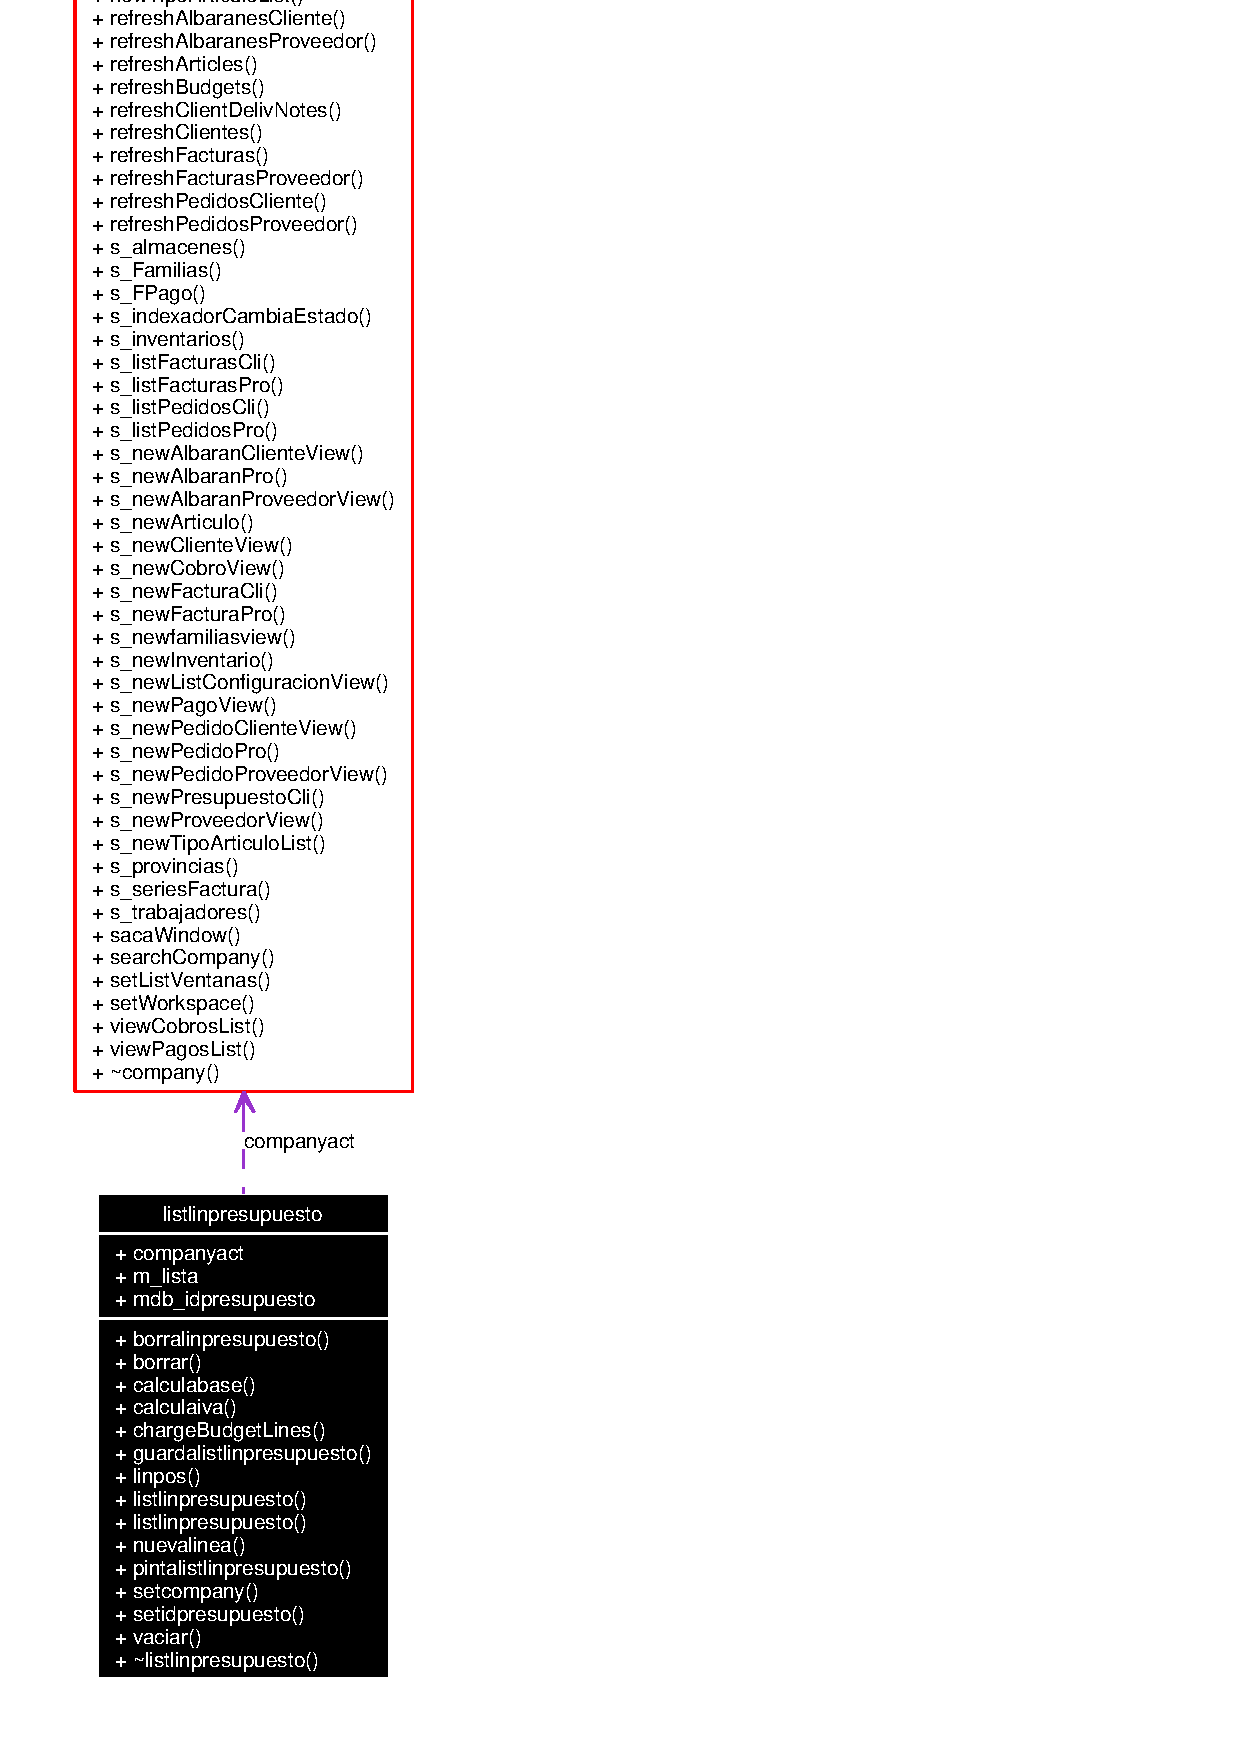
\includegraphics[width=99pt]{classlistlinpresupuesto__coll__graph}
\end{center}
\end{figure}
\subsection*{M\'{e}todos p\'{u}blicos}
\begin{CompactItemize}
\item 
void {\bf borralinpresupuesto} (int)\label{classlistlinpresupuesto_a0}

\item 
void {\bf borrar} ()\label{classlistlinpresupuesto_a1}

\item 
float {\bf calculabase} ()\label{classlistlinpresupuesto_a2}

\item 
float {\bf calculaiva} ()\label{classlistlinpresupuesto_a3}

\item 
int {\bf charge\-Budget\-Lines} (QString)
\begin{CompactList}\small\item\em Carga l\'{\i}neas de presupuesto. \item\end{CompactList}\item 
void {\bf guardalistlinpresupuesto} ()\label{classlistlinpresupuesto_a5}

\item 
{\bf linpresupuesto} $\ast$ {\bf linpos} (int)\label{classlistlinpresupuesto_a6}

\item 
{\bf listlinpresupuesto} ({\bf company} $\ast$comp)\label{classlistlinpresupuesto_a8}

\item 
void {\bf nuevalinea} (QString, QString, QString, QString, QString, QString, QString, QString)\label{classlistlinpresupuesto_a9}

\item 
virtual void {\bf pintalistlinpresupuesto} ()\label{classlistlinpresupuesto_a10}

\item 
void {\bf setcompany} ({\bf company} $\ast$c)\label{classlistlinpresupuesto_a11}

\item 
void {\bf setidpresupuesto} (QString id)\label{classlistlinpresupuesto_a12}

\item 
void {\bf vaciar} ()\label{classlistlinpresupuesto_a13}

\end{CompactItemize}
\subsection*{Atributos p\'{u}blicos}
\begin{CompactItemize}
\item 
{\bf company} $\ast$ {\bf companyact}\label{classlistlinpresupuesto_o0}

\item 
QList$<$ {\bf linpresupuesto} $\ast$ $>$ {\bf m\_\-lista}\label{classlistlinpresupuesto_o1}

\item 
QString {\bf mdb\_\-idpresupuesto}\label{classlistlinpresupuesto_o2}

\end{CompactItemize}


\subsection{Descripci\'{o}n detallada}
Administra las l\'{\i}neas de detalle de un presupuesto. 



\subsection{Documentaci\'{o}n de las funciones miembro}
\index{listlinpresupuesto@{listlinpresupuesto}!chargeBudgetLines@{chargeBudgetLines}}
\index{chargeBudgetLines@{chargeBudgetLines}!listlinpresupuesto@{listlinpresupuesto}}
\subsubsection{\setlength{\rightskip}{0pt plus 5cm}int listlinpresupuesto::charge\-Budget\-Lines (QString {\em idbudget})}\label{classlistlinpresupuesto_a4}


Carga l\'{\i}neas de presupuesto. 

Creamos un elemento del tipo linpresupuesto y lo agregamos a la lista.

Tratamiento de excepciones. 

La documentaci\'{o}n para esta clase fu\'{e} generada a partir de los siguientes archivos:\begin{CompactItemize}
\item 
listlinpresupuesto.h\item 
listlinpresupuesto.cpp\end{CompactItemize}
